\documentclass[sigconf]{acmart}
\settopmatter{printacmref=false}

\renewcommand\footnotetextcopyrightpermission[1]{}

\pagestyle{plain}

\usepackage{supertabular,booktabs,float}
%\usepackage[textheight=10cm]{geometry}   %% just for this example.





\begin{document}
\title{Computational Intelligence Coursework}
\acmConference[SET10107]{Coursework}{April 2018}{Edinburgh Napier University} 
\acmYear{2018}
\copyrightyear{2018}

\author{40200819}



\begin{abstract}
This report details the development of an evolutionary algorithm that evolves the weights of a neural network. The selection, crossover and replacement methods are discussed, including why they were chosen and the parameters used to make them work effectively. The experiments and analysis section then explores how the algorithm was changed based on experimentation to reduce fitness scores. The conclusions and future work sections discuss what was gained from the project and what could be done to further improve the algorithm in the future.
\end{abstract}



%\keywords{ACM proceedings, \LaTeX, text tagging}


\maketitle

\section{Introduction}
Evolutionary algorithms allow us to find good solutions to problems that don't necessarily have answers yet, in a process similar to biological evolution \cite{evoAlgIntro}. A population is initialised randomly and each member's fitness, a function of their ability to solve the problem, is evaluated. Measuring and evaluating the fitness of each attempt allows the algorithm to select and breed (crossover) the better ones to create children - an exploitation of the best members in the population \cite{exploreExploit}. Mutation allows the algorithm to explore new options by changing genes by a certain amount, according to a predetermined chance variable. Finally, the worst members of the population are replaced with the newly created children. Running the algorithm multiple times allows it to approach a solution - in this case a set of weights for a neural network - that can ideally also work well on a new 'test' data set.

The algorithm developed alongside this report is built from the example evolutionary algorithm provided with the coursework project template. This report will refer to solutions by number, in order of their creation - eg: 'Solution One'. These solutions are explored in depth in the Experiments \& Analysis section.

\section{Approach}
This algorithm incorporates evolutionary programming to land rockets on a pad in a simulated environment, whilst trying to use as much fuel as possible. This is done by evolving the weights of a neural network, which is then used to control the rockets. 

The goal of this project was to design an appropriate evolutionary algorithm that could reduce the fitness enough to get good results on the test data set without overfitting to the training set \cite{overfitting}.

The following subsections describe the algorithm's various operators in detail, including why they were used and what parameters were chosen to optimise them.

\subsection{Selection}
When choosing a selection method, various options were researched including roulette and rank selection. Tournament selection was chosen as it appeared to be the simplest to start with and provided a good benchmark to build from. Tournament selection works by choosing a random group of members from the population and then picking the best one from the group \cite{tournament3}. This gives every member of the population a chance of being chosen, which should maintain diversity \cite{tournament} and naturally provides rank based selection for a low computational cost \cite{tournament2}.

The number of members competing in each tournament is known as the tournament size. The author experimented with this value, finding a tournament size of 8 to be the best. This may be because a high tournament size increases selection pressure, which allows the algorithm to quickly converge on a good solution within the 20000 evaluations limit \cite{selectionPressure}. This could be optimised in the future by running a full scientific test on the algorithm with multiple tournament sizes to find the best possible tournament size. The author attempted to do this early in the project (before the creation of solution one) but unfortunately saw no correlation between tournament size and fitness, possibly because of other factors such as low mutation values and an unoptimised algorithm. This experiment can be seen in the graph below. Each tournament size had 5 runs, with the average fitness across all of them recorded on the graph.

\begin{figure}[H]
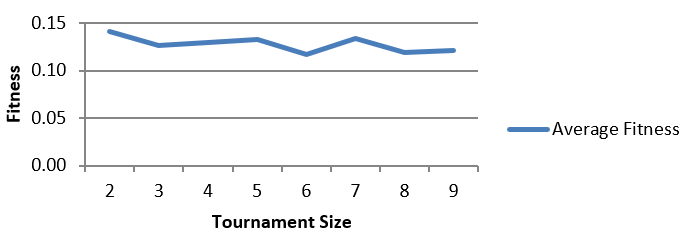
\includegraphics[width=\columnwidth]{useless.png}
\caption[width=\columnwidth]{This experiment, conducted early in the process, didn't help to find a good tournament size} \label{Useless}
\end{figure}

Initially, tournament contenders were chosen randomly from the population as is standard for tournament selection \cite{tournament3}. This worked fine, but the author decided to adjust this to improve the chance of a good parent being selected. This was accomplished by ordering the population from highest to lowest fitness and requiring the participants to be within the best 75\% of the population. The author found that this improved overall fitness whilst not negatively impacting the diversity of the population.

\subsection{Crossover}
Crossover is the process of combining the genes of 2 or more parent chromosomes to make a new child chromosome. To start with, the algorithm used single point crossover at a random position as it allows each parent an equal chance to influence the child's genes. This means that the child's chromosome was split in two, with the first section being based on the first parent's genes and the second section based on the other parent's genes \cite{singlePoint}.

This was later changed to a multi-point crossover solution, where crossover points are placed at regular intervals based on the number of parents involved in the crossover - taking a segment of each parent's genes for the child. This adjustment allowed the algorithm to work with any number of parents. This was based on \cite{multipleParents}, which suggests that breeding more than 2 parents at once can create greater diversity.

This new approach was indeed successful at increasing diversity, but having more than 2 parents increased fitness overall, possibly because the best parents were drowned out. As a result of this, solution one reduced the number of parents back to 2, with the option to increase it again for future solutions.
\subsection{Replacement}
The replace-worst strategy used by this algorithm is relatively simple; it always replaces the worst member of the population with each new child generated, unless the new child is even worse. This was chosen to rapidly improve the population, but requires a large population size as a smaller population would converge too quickly under this replacement scheme \cite{replacement}.

Initially, the algorithm always replaced the worst in the population with the new child, even if the new child's fitness was even worse. In theory, this should have increased diversity in the population, but it was ultimately removed as it slowed down the algorithm with too much backtracking and the diversity wasn't increased enough to be worth it.

As the worst member of the population will be quickly replaced, the author decided to mutate it first, just in case it becomes a better solution worth keeping. To do this, a copy of the worst member is mutated and then run through the replacement operator as if it were a new child. It will either mutate for the better and replace it's original state, or it will be discarded if mutation makes it worse. At first, this used the mutation rate, but the author decided to mutate the worst one every time to increase the chance of a good mutation.

\subsection{Parameters}
Early on in the project, the author achieved great results with a mutation rate of 0.5 and a mutation change of 0.2. These values created some excellent fitness results and even landed all 180 rockets in the test set on one occasion. Unfortunately, according to \cite{mutateRate}, a high mutation rate can potentially damage the fitness of the best members of the population by mutating too much at once and missing the best solutions. Therefore, the author worked to achieve similar results with lower mutation values by improving the algorithm and adjusting other parameters. 

For solution one, the mutation rate was set to 0.5 and the mutation change to 0.12. These were eventually revised to a more even 0.2 for both values in solution four. This adjustment made the mutation change a factor of the minimum and maximum gene values, which are -1 and +1 respectively - allowing the full range to be explored.

According to \cite{hiddenLayers}, the number of hidden layers should be 1 for most problems and the number of nodes per hidden layer should be between the number of input nodes (5 in our case) and the number of output nodes (3 in our case). Following this rule, 4 is the optimal amount and therefore is the amount chosen for this algorithm.

The population size was changed multiple times as part of the algorithm's development, settling on 80 by solution four. More details on the changes to this parameter can be found in the Experiments \& Analysis section.

\section{Experiments \& Analysis}
The algorithm was initially tested by running it in the GUI and watching to see how well it performed on the graph. This approach allowed the author to quickly evaluate the results and make changes. 

The author created a solution to use as a benchmark for further improvement. This solution, referred to as solution one in this report, was the result of some initial experimentation and reading to get a good baseline to build from.

The table below shows the results of solution one across 10 runs of the algorithm. The average and best fitness values are from the training set, whilst 'fitness with test' referrers to the average fitness when applied to the test set.

\tablefirsthead{\toprule \begin{tabular}{@{}p{0.1\columnwidth}p{0.25\columnwidth}p{0.25\columnwidth}p{0.25\columnwidth}}
Run&Average Fitness&Best Fitness&Fitness with test
\end{tabular}\\ \midrule}
%
\tablehead{%
\multicolumn{4}{r}%
{{\bfseries  Continued from previous column}} \\
\toprule
\begin{tabular}{@{}p{0.1\columnwidth}p{0.25\columnwidth}p{0.25\columnwidth}p{0.25\columnwidth}}
Run&Average Fitness&Best Fitness&Fitness with test
\end{tabular}\\ \midrule}
%
\tabletail{%
    \midrule
    \multicolumn{4}{r}{{Continued on next column}}
    \midrule
}
\tablelasttail{
    \hline
    \multicolumn{4}{c}{{\textbf{Table 1: Solution One}}}
}
\begin{supertabular}{@{}p{0.1\columnwidth}p{0.25\columnwidth}p{0.25\columnwidth}p{0.25\columnwidth}}
    1&0.11851819&0.109464577&0.258081383\\
    2&0.028939944&0.015180927&0.017754965\\
    3&0.04011759&0.02400237&0.035088488\\
    4&0.057333324&0.017464973&0.019361096\\
    5&0.07832602&0.055195203&0.182122002\\
    6&0.10133906&0.083893989&0.219561067\\
    7&0.031817164&0.019409874&0.020543711\\
    8&0.041717841&0.021008549&0.035884758\\
    9&0.055988408&0.042648306&0.105620024\\
    10&0.115002294&0.11015399&0.22500339\\
    Range&0.089578246&0.094973063&0.240326418\\
    Average&0.066909984&0.049842276&0.11190208\\
    
\end{supertabular}%
\\

As shown below, the best fitness graphs from solution one typically resemble a cotangent curve; fitness decreases very rapidly at the start, slowing down in the middle and then rapidly decreases again towards the end. This is an issue as occasionally the second decline started too late and would not reach a good fitness before the evaluation limit was reached.

\begin{figure}[H]
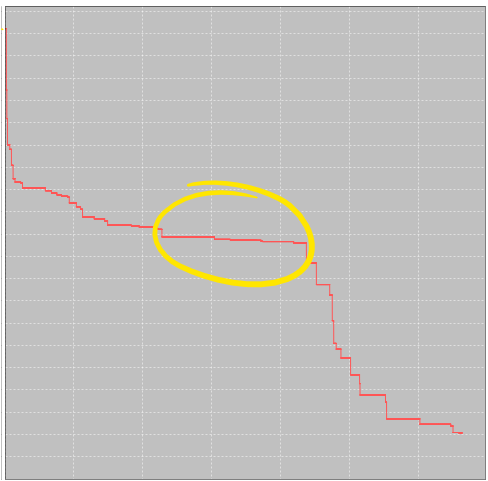
\includegraphics[width=\columnwidth]{SolOneGraph.png}
\caption[width=\columnwidth]{Solution One slows down in the middle} \label{SolOneGraph}
\end{figure}

One of the goals for future solutions was to aim for an exponentially decreasing curve, which should allow for more progress in the same number of evaluations.

The range of results for each solution was recorded, which helped the author tune the results for consistency. This was done using a box plot for the average fitness, best fitness and test fitness.

The figure below shows solution one's box plot, which indicates a very wide range of results.

\begin{figure}[H]
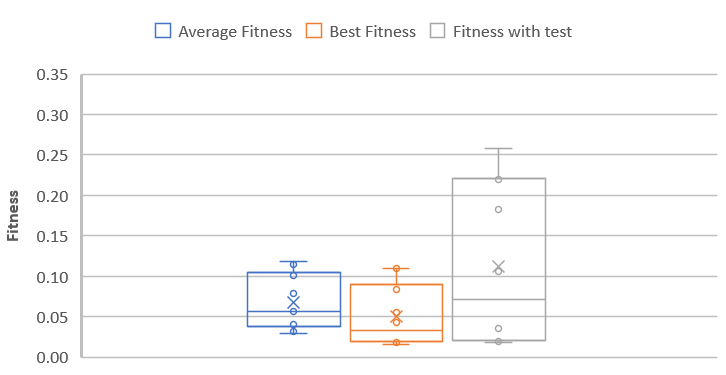
\includegraphics[width=\columnwidth]{SolOneBox.png}
\caption[width=\columnwidth]{Solution One has a very wide range of results, making it unpredictable} \label{SolOneBox}
\end{figure}

The boxplots use an X to indicate the mean and a line to indicate the median. Solution one has a large spread of results, with an average fitness Inter Quartile Range of approximately 0.038 to 0.105. This makes the results quite inconsistent, with the test dataset's results having a huge IQR of roughly 0.02 to 0.221.

The population size was modified many times when trying to create solution one, settling on a size of 40. As shown above, the first solution had a very wide range of results. The author theorised that this was due to the large population not changing fast enough, causing the breeding of bad parents, which slowed the overall improvement of the population.

To counteract this, solution two halved the population for a size of 20, aiming to fix the range issue. Unfortunately, whilst this adjustment helped reduce the variance of the results, the average fitness actually increased for all three metrics (average, best and test dataset) as shown in table 2 below.

\tablefirsthead{\toprule \begin{tabular}{@{}p{0.1\columnwidth}p{0.25\columnwidth}p{0.25\columnwidth}p{0.25\columnwidth}}
Run&Average Fitness&Best Fitness&Fitness with test
\end{tabular}\\ \midrule}
%
\tablehead{%
\multicolumn{4}{r}%
{{\bfseries  Continued from previous column}} \\
\toprule
\begin{tabular}{@{}p{0.1\columnwidth}p{0.25\columnwidth}p{0.25\columnwidth}p{0.25\columnwidth}}
Run&Average Fitness&Best Fitness&Fitness with test
\end{tabular}\\ \midrule}
%
\tabletail{%
    \midrule
    \multicolumn{4}{r}{{Continued on next column}}
    \midrule
}
\tablelasttail{
    \hline
    \multicolumn{4}{c}{{\textbf{Table 2: Solution Two}}}
}
\begin{supertabular}{@{}p{0.1\columnwidth}p{0.25\columnwidth}p{0.25\columnwidth}p{0.25\columnwidth}}
    1&0.034153283&0.015601448&0.036587929\\
    2&0.050594412&0.026087938&0.089452558\\
    3&0.105339055&0.101256037&0.224750837\\
    4&0.073032603&0.06089453&0.106926161\\
    5&0.06987493&0.055993985&0.143814427\\
    6&0.114281346&0.108934445&0.227398511\\
    7&0.112070438&0.105234741&0.211971992\\
    8&0.029143217&0.015727459&0.025050597\\
    9&0.102454038&0.080581761&0.208346109\\
    10&0.032861951&0.016624956&0.037528336\\
    Range&0.085138129&0.093332996&0.202347914\\
    Average&0.072380527&0.05869373&0.131182746\\
    
\end{supertabular}%
\\
This increase in overall fitness is likely because there was not enough diversity in the population.

To confirm this theory, two small tests were conducted named solution two B and solution two C. B halved the population again, and after 5 runs, it further decreased the range and increased the average fitness. This solution was not be explored further as the average fitness was too high and the change in range very minimal.

Solution two C went the other way and doubled the population size from solution one's 40 to 80. This was very interesting as the range still decreased, and by a larger amount, whilst also decreasing the average fitness.

This result was surprising, according to the trend of the previous experiments, increasing the population should have made the range of results wider. A possible explanation for this was a small change to the algorithm: At this point, the author had realised that the worst member was not mutated at every evaluation, instead only mutating according to the mutation rate. To delay fixing this, the 'worst member' mutation function had been disabled temporarily.

To confirm that it was the population size that created this improvement and not the adjusted algorithm, the author created a new test, named solution two D, which would revert the algorithm back to it's state in solution one, with only the population size changed.

Solution Two D performed very well, with similar results to solution two C despite the algorithm changes. This suggested that a population of 80 was definitely an improvement.

At this point, the author created solution three, with a population of 80 and with the 'worst mutated' concept correctly implemented to always mutate the worst one in the data set regardless of the mutation rate. 

This solution provided the best results yet, decreasing all of the fitness metrics by a considerable amount and drastically reducing the range, as shown in table 3 below.

\tablefirsthead{\toprule \begin{tabular}{@{}p{0.1\columnwidth}p{0.25\columnwidth}p{0.25\columnwidth}p{0.25\columnwidth}}
Run&Average Fitness&Best Fitness&Fitness with test
\end{tabular}\\ \midrule}
%
\tablehead{%
\multicolumn{4}{r}%
{{\bfseries  Continued from previous column}} \\
\toprule
\begin{tabular}{@{}p{0.1\columnwidth}p{0.25\columnwidth}p{0.25\columnwidth}p{0.25\columnwidth}}
Run&Average Fitness&Best Fitness&Fitness with test
\end{tabular}\\ \midrule}
%
\tabletail{%
    \midrule
    \multicolumn{4}{r}{{Continued on next column}}
    \midrule
}
\tablelasttail{
    \hline
    \multicolumn{4}{c}{{\textbf{Table 3: Solution Three}}}
}
\begin{supertabular}{@{}p{0.1\columnwidth}p{0.25\columnwidth}p{0.25\columnwidth}p{0.25\columnwidth}}
    1&0.051645209&0.027799086&0.05979013\\
    2&0.08541211&0.060828927&0.142983012\\
    3&0.031970246&0.017267509&0.025337601\\
    4&0.071116378&0.039464773&0.189740275\\
    5&0.065617239&0.041982113&0.127582698\\
    6&0.091730571&0.067899694&0.215405856\\
    7&0.110470171&0.106707586&0.234569601\\
    8&0.08806873&0.071138477&0.200138552\\
    9&0.098184532&0.065608281&0.149567704\\
    10&0.037651284&0.01474351&0.057182944\\
    Range&0.053441863&0.043561418&0.164402674\\
    Average&0.061152236&0.037468482&0.109086743\\
    
\end{supertabular}%
\\

At this point, the population size was quite large and there were other variables that hadn't been altered. These included the mutation rate and mutation change parameters that were 0.5 and 0.12 respectively.

As the gene sizes were limited between the values of -1 and +1, it made sense to have a mutation change that was a factor of this limit, allowing the genes to mutate all the way to the maximum and minimum values. For this reason, the mutation change was set to a value of 0.2.

As mentioned in section 2.4, the author wanted to limit the mutation values as much as possible without harming results. After a bit of experimentation, a mutation rate of 0.2 was chosen.

These new values formed solution four. See the table below for the values produced by this solution.

\tablefirsthead{\toprule \begin{tabular}{@{}p{0.1\columnwidth}p{0.25\columnwidth}p{0.25\columnwidth}p{0.25\columnwidth}}
Run&Average Fitness&Best Fitness&Fitness with test
\end{tabular}
\\ \midrule}
%
\tablehead{%
\multicolumn{4}{r}%
{{\bfseries  Continued from previous column}} \\
\toprule
\begin{tabular}{@{}p{0.1\columnwidth}p{0.25\columnwidth}p{0.25\columnwidth}p{0.25\columnwidth}}
Run&Average Fitness&Best Fitness&Fitness with test
\end{tabular}\\ \midrule}
%
\tabletail{%
    \midrule
    \multicolumn{4}{r}{{Continued on next column}}
    \midrule
}
\tablelasttail{
    \hline
    \multicolumn{4}{c}{{\textbf{Table 4: Solution Four}}}
}
\begin{supertabular}{@{}p{0.1\columnwidth}p{0.25\columnwidth}p{0.25\columnwidth}p{0.25\columnwidth}}
    1&0.035568813&0.015935681&0.031763971\\
    2&0.029870228&0.018154525&0.023431724\\
    \textbf{3}&\textbf{0.12670661}&\textbf{0.123122264}&\textbf{0.333836236}\\
    4&0.05261057&0.029927838&0.052549836\\
    5&0.04825385&0.022454602&0.091233089\\
    6&0.027969792&0.01809619&0.031091275\\
    7&0.048717748&0.023970202&0.073158761\\
    8&0.071666729&0.045946377&0.133108958\\
    9&0.068078789&0.046473026&0.129392741\\
    10&0.082394627&0.057726208&0.145349429\\
    Range&0.096836381&0.107186583&0.310404512\\
    Average&0.058602014&0.041918982&0.106562971\\
    
\end{supertabular}%
\\

At first, this solution appears to be worse than solution three in every way except for average and test fitness, with the range being particularly large. However, the outlier (highlighted in bold on the table) is heavily skewing the results. This solution actually produced much better results overall, which is made clear when comparing the box plots of the two solutions.

\begin{figure}[H]
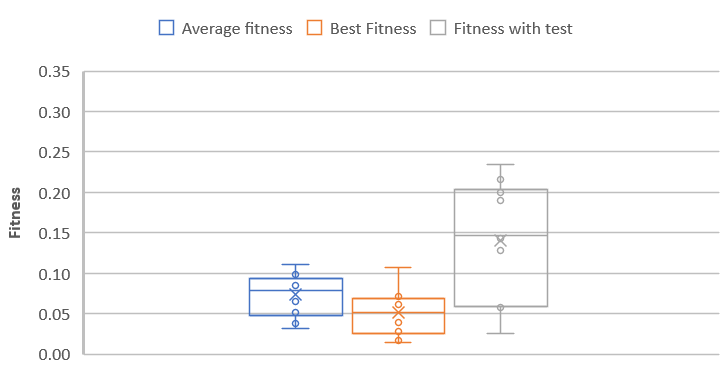
\includegraphics[width=\columnwidth]{SolThreeBox.png}
\caption[width=\columnwidth]{Solution Three has no outliers, but worse results overall} \label{SolThreeBox}
\end{figure}

\begin{figure}[H]
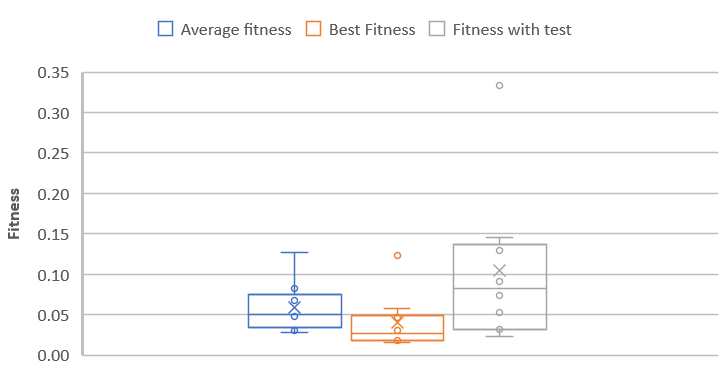
\includegraphics[width=\columnwidth]{SolFourBox.png}
\caption[width=\columnwidth]{Solution Four has a very prominent outlier, but otherwise much improved results} \label{SolFourBox}
\end{figure}

As shown by the line that goes through the box plots, the median value is much lower for solution four across the board. The inter-quartile range is also much smaller. Therefore, it seems that solution four is an improvement overall despite the outlier.

At this point the project time was nearly over, ideas for further improvement of the algorithm are in section 5.

The following graphs plot the solutions against each other, with each solution as a different series. This approach allows each solution to be compared easily and also reduces the risk of bad outliers skewing results by showing each run individually.

\begin{figure}[H]
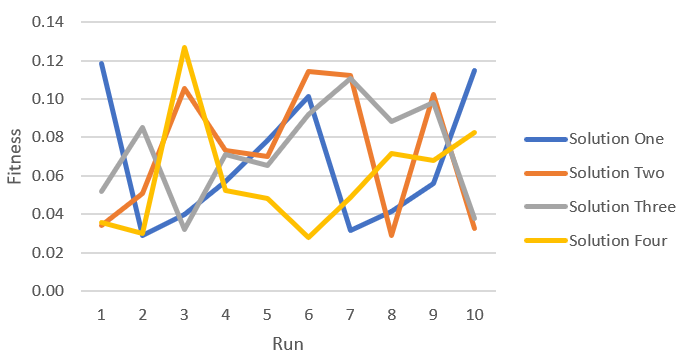
\includegraphics[width=\columnwidth]{averageFitnessAll.png}
\caption[width=\columnwidth]{Average fitness of each solution for all 10 runs} \label{avFitAll}
\end{figure}

This first graph shows that two solutions clearly stand out, solution one and solution four. Solution one gets some very good results in some areas, for example run 7, where it does better than all of the others. However, solution one frequently does quite badly, with runs 1, 5, 6 and 10 being examples.

In contrast, solution four has the highest peak of the whole graph in run 3, but otherwise does very well, with consistent results.

These results make it clear that solution three was actually worse than solution one in some ways, as it frequently has a higher fitness such as in runs 2, 4, 7, 8 and 9. Figure \ref{SolThreeBox} does show that solution three's median was higher than that of solution one, but it also shows the reduced range of results that is less obvious from figure \ref{avFitAll} above.

The next graph shows the best fitness of each of the solutions for every run.

\begin{figure}[H]
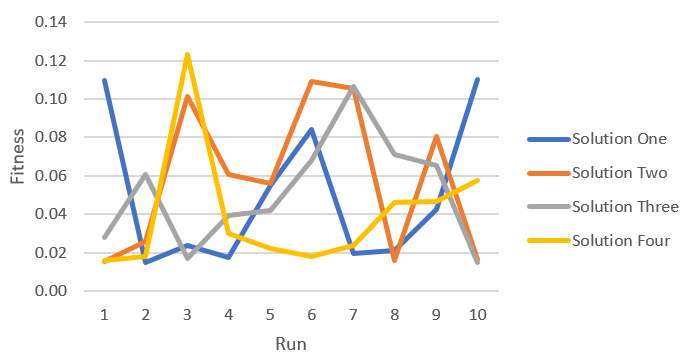
\includegraphics[width=\columnwidth]{bestFitnessAll.png}
\caption[width=\columnwidth]{Best fitness of each solution for all 10 runs} \label{bestFitAll}
\end{figure}

This graph is very similar to figure \ref{avFitAll}, though there is one key point to bring up: The best fitness lines almost exactly match the average fitness lines, suggesting that the best fitness has a close relation to the fitness of the whole population. This could be a sign that there isn't enough diversity in any of the solutions.

The final graph below shows the fitness with the test data set for each solution.

\begin{figure}[H]
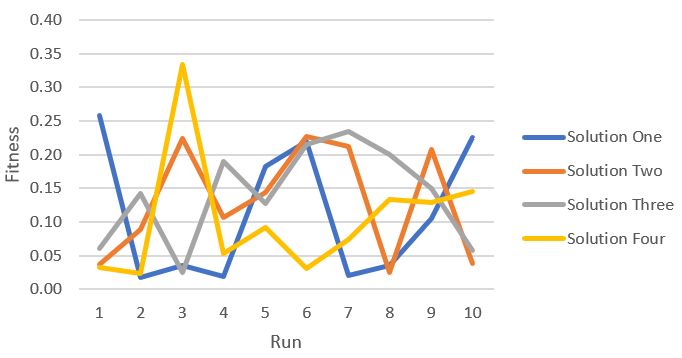
\includegraphics[width=\columnwidth]{testFitnessAll.png}
\caption[width=\columnwidth]{Test fitness of each solution for all 10 runs} \label{bestFitAll}
\end{figure}

The scale on this graph is much larger, but this allows us to see the relation between the best fitness on the training set versus the fitness on the test set. As expected, all of the results are similar to the previous two graphs with solution four being better than the others in most cases.

Figure \ref{exponential} below shows what an average run looks like with solution four. It still has a cotangent curve at times, but often has the desired exponential shape. This indicates that solution four makes effective use of the 20000 evaluations it completes, with minimal downtime.

\begin{figure}[H]
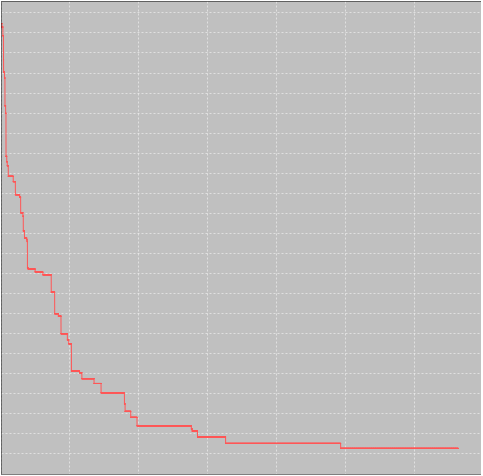
\includegraphics[width=\columnwidth]{Exponential.png}
\caption[width=\columnwidth]{Solution Four reduces fitness at a much more consistent pace than solution one} \label{exponential}
\end{figure}

\section{Conclusions}
This project was quite challenging as it required a lot of experimentation to find good results. Solution one represents the first instance of good results, with the other three solutions representing refinements based on scientific analysis. The table below details solution four, including the fitness values and the activation function used by the neural network.

\tablefirsthead{\toprule \begin{tabular}{@{}p{0.1\columnwidth}p{0.15\columnwidth}p{0.05\columnwidth}p{0.1\columnwidth}p{0.1\columnwidth}p{0.1\columnwidth}p{0.1\columnwidth}}
Set&Average/ Best Fitness&Pop Size&Mut. Rate/ Change&Hidden Nodes&Min/ Max gene&Activation function
\end{tabular}
\\ \midrule}
%
\tablelasttail{
    \hline
    \multicolumn{7}{c}{{\textbf{Table 5: }Details of the final solution}}
}
\begin{supertabular}{@{}p{0.1\columnwidth}p{0.15\columnwidth}p{0.05\columnwidth}p{0.1\columnwidth}p{0.1\columnwidth}p{0.1\columnwidth}p{0.1\columnwidth}}
    Training&0.058602014 0.01809619&80&0.2/0.2&4&-1/+1&Step\\
    Test&0.106562971 0.023431724&80&0.2/0.2&4&-1/+1&Step\\
    
\end{supertabular}%
\\

This project was successful as the average and best fitness values were reduced substantially from the original solution. The range of results was also reduced, making the results more reliable.

The experiments and analysis conducted for this project made clear which properties had the most bearing on the project. The population size made a huge difference to the project, with a bigger population allowing for more diversity and better results overall.

Other conclusions can be drawn from the use of mutation rate and mutation change. As mentioned, the author managed to land all 180 rockets by upping these parameters to extreme levels, so these parameters have a large impact on the fitness, but shouldn't be over used as they can cause the best solutions to be skipped over. Also, the mutation change should be a factor of the minimum/maximum gene values.

Having lots of parents for crossover may create greater diversity, but at the cost of diluting the best parent's genes with each parent added. The crossover implementation worked better when using a fixed crossover point as opposed to a random one, which was interesting as a random crossover point seems to be standard practice \cite{singlePoint}.

It is important to pay attention to the median of a dataset when comparing it to others, as was the case in solution three, which was actually worse than solution one in some ways - median being one of them. Similarly, large outliers can skew a dataset and make a solution look worse on average; showing each run individually is a good way to avoid this issue.

As discussed in section 2, the tournament selection method was chosen due to it's simplicity, with the intention to go back to it should the algorithm not perform well. Of course, comparisons between these algorithms do exist already in literature, but they are often used in different circumstances and contexts, which were hard to apply to this algorithm. 

Therefore, the best way to scientifically compare selection methods such as roulette and tournament would be swapping the selection method within solution four and recording the results. This would allow direct comparison between the methods in the context of the existing solution, without the risk of other factors interfering with the outcome.
\section{Future work}
There are variables and concepts that haven't been explored in this project that could improve the algorithm even further, ideally reducing the fitness to 0.01 or lower. The range could also be reduced to decrease the chance of a bad run or an extreme outlier.

As mentioned in section 2.2, more than 2 parents in each crossover is already possible with the algorithm and could be experimented with in the future. This could be accompanied with a more complex type of crossover such as gene scanning, diagonal crossover \cite{multiParent2} or SPX \cite{multipleParents} that is specifically designed for 3 or more parents, rather than the multi-point crossover attempted in this project.

Another area that wasn't fully explored was the mutation of the worst member of the population. What if more were mutated at once, such as the top 5 highest fitness? This could be particularly relevant if the population was increased beyond 80, as just mutating one bad member per evaluation will have less of an impact as the population size increases.

Increasing the population further may also improve results as the highest population size tested was 80, the size that the final solution uses. This would need to be increased with caution, as according to \cite{popSize} 'If the population is too large . . . undesired computational resources may be incurred and the waiting time for a fitness improvement may be too long'. The same article discusses the use of a dynamic population size, which may be another avenue for improvement.

The mutation, initialisation and activation functions were all left unaltered by this project (Except for a small tweak to allow the worst member to ignore the mutation rate). These could be investigated to improve results further in the future.

\bibliographystyle{ACM-Reference-Format}
\bibliography{Bibliography} 

\end{document}
